\documentclass{article}
\usepackage[utf8]{inputenc}
\usepackage{amsmath}
\usepackage[linesnumbered,ruled]{algorithm2e}
\usepackage{mathtools}
\usepackage{commath}
\usepackage{tikz}
\usetikzlibrary{shapes.geometric, arrows}

\title{Xenobot technical report}
\author{Shengwen Cheng}
\date{January 2017}

\begin{document}

\maketitle

\tikzstyle{blocks} = [rectangle, rounded corners, minimum width=2cm, minimum height=1cm,text centered, draw=black, fill=orange!30]
\tikzstyle{arrow} = [thick,->,>=stealth]

\section{Introduction}
Xenobot is a computer vision based self-driving system inspired by MIT duckietown project. We hope to do the real-time robotics research or add new customized functions after re-implementing the system.
\\
\\
The algorithm we are using is a modified version of MIT duckietown, so you can find many similarities between two projects. This report is focus on how our lane following algorithm works.
\\
\\
\\
\\

\begin{figure} [h!]
  \centering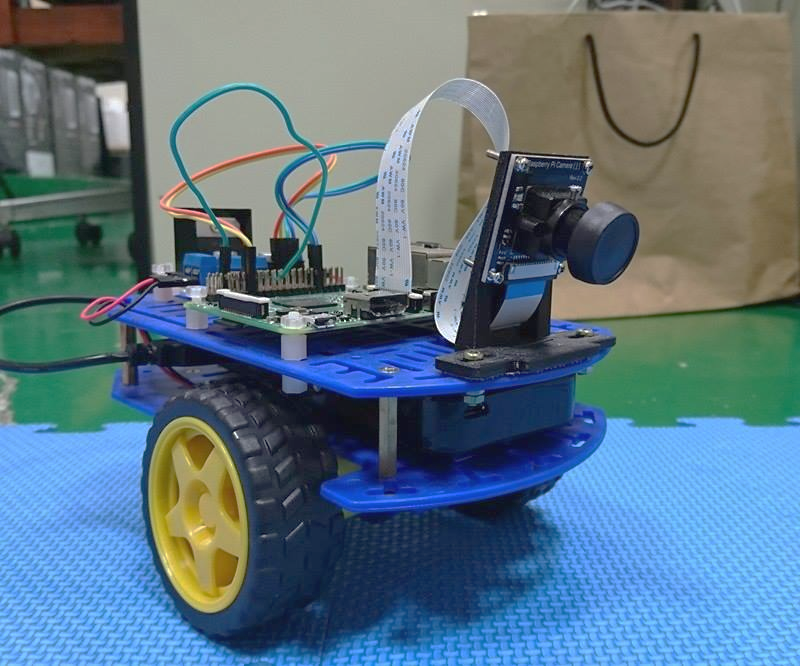
\includegraphics[scale=0.3]{xenobot.png}
  \caption{Xenobot}
\end{figure}


\section{Lane pose estimation}

\subsection{Assumptions of the environment}
\begin{figure} [ht]
  \centering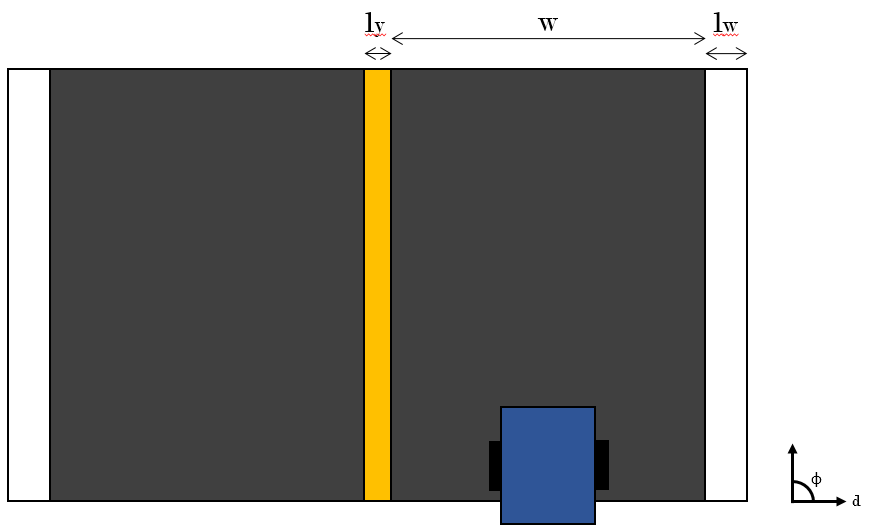
\includegraphics[scale=0.5]{lane.png}
  \caption{lane}
\end{figure}


\subsection{Segements detection}
\begin{figure} [ht]
\begin{center}
\begin{tikzpicture}[node distance=2cm]
\node (raw) [blocks, yshift=0cm] {Raw image} ;
\node (rectify) [blocks, yshift=-1.5cm] {Distortion and rectification};
\node (canny) [blocks, xshift=-2cm, yshift=-3cm] {Canny edge detection};
\node (diliation_canny) [blocks, xshift=-2cm, yshift=-4.5cm] {Diliation};
\node (threshold) [blocks, xshift=2cm, yshift=-3cm] {HSV color thresholding};
\node (diliation_threshold) [blocks, xshift=2cm, yshift=-4.5cm] {Diliation};
\node (and) [blocks, yshift=-6cm] {Bitwise And};
\node (hough) [blocks, yshift=-7.5cm] {Hough transform};
\node (segments) [blocks, yshift=-9cm] {Segments};

\draw [arrow] (raw) -- (rectify);
\draw [arrow] (rectify) -- (canny);
\draw [arrow] (canny) -- (diliation_canny);
\draw [arrow] (rectify) -- (threshold);
\draw [arrow] (threshold) -- (diliation_threshold);
\draw [arrow] (diliation_canny) -- (and);
\draw [arrow] (diliation_threshold) -- (and);
\draw [arrow] (and) -- (hough);
\draw [arrow] (hough) -- (segments);
\end{tikzpicture}
\end{center}
\caption{Work flow of lane detector}
\end{figure}




\subsection{Coordinate transformation}
\begin{figure} [ht]
  \centering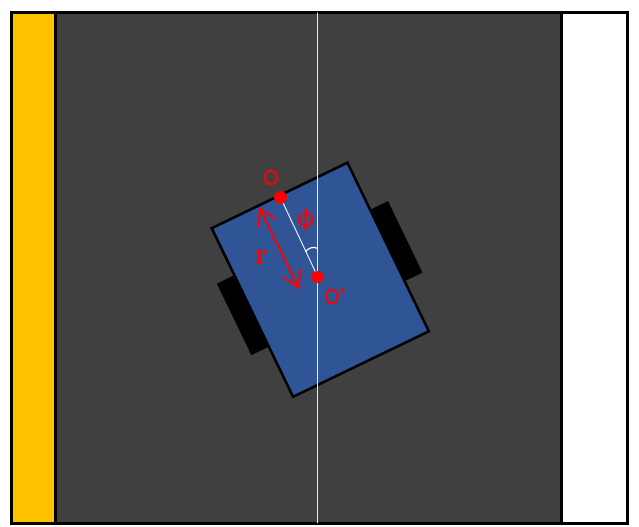
\includegraphics[scale=0.5]{car_center.png}
  \caption{Center of camera and the car}
\end{figure}

\begin{figure} [h!]
  \centering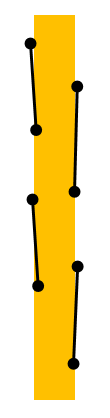
\includegraphics[scale=0.5]{edge_side.png}
  \caption{segment side}
\end{figure}

\subsection{Segment side recognition}
We obtained the lane segments during the lane detection process. Next step to do is to figure out the side of the segment on the lane mark. We can determine it by reading multiple pixel values in the direction of the segment normal vector on the color thresholding image.
\begin{figure} [ht]
\begin{algorithm}[H]
	\KwData{segment, accumulator threshold, color binarization image}
	\KwResult{side (left or right)}
	$\vec{P_1} = (x_1, y_1)$
	\\
	$\vec{P_2} = (x_2, y_2)$
	\\
	$\vec{P} = \frac{\vec{P_1} + \vec{P_2}}{2}$
	\\
	$\vec{t} = \frac{\vec{P_2} - \vec{P_1}}
					{\norm{\vec{P_2} - \vec{P_1}}}$
	\\
	$\vec{n} = (-y_t, x_t)$
	\\
	\For {$i < pixel \ count$} {
		$x \gets \lceil x_p + x_n \cdot i \rceil$
		\\
		$y \gets \lceil y_p + y_n \cdot i \rceil$
		\\		
		\uIf{$I(x,y) = I_{max}$}
			{
				$left \gets left + 1$ 
			}
			
		$x \gets \lfloor x_p - x_n \cdot i \rfloor$
		\\
		$y \gets \lfloor y_p - y_n \cdot i \rfloor$
		\\		
		\uIf{$I(x,y) = I_{max}$}
			{
				$right \gets right + 1$ 
			}
	}
	
	\uIf {$left > threshold \ \& \  right < threshold$}
		{
			\Return is left
		}
	\uElseIf {$right > threshold \ \& \ left < threshold$}
		{
			\Return is right
		}
	\uElse
		{
			\Return unknown side
		} 
	\caption{Segment side recognition}
\end{algorithm}
\end{figure}

\subsection{Lane pose estimation for single segment}
\begin{figure} [ht]
  \centering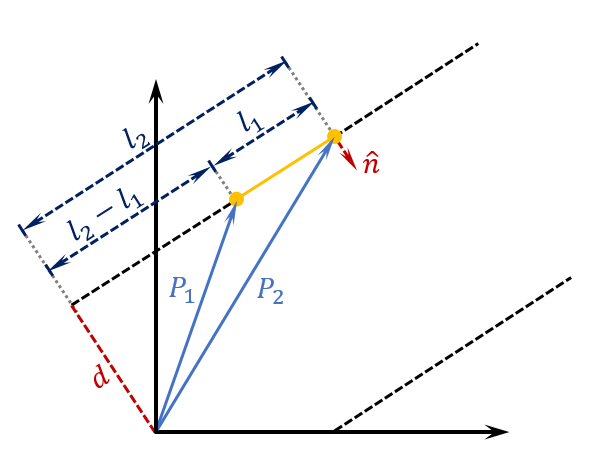
\includegraphics[scale=0.9]{pose_explain.png}
  \caption{Geometry relationships}
\end{figure}

\begin{figure} [ht]
\begin{algorithm}[H]
	\KwData{segment}
	\KwResult{pose $d$ and $\phi$}
	$\vec{P_1} = (x_1, y_1)$
	\\
	$\vec{P_2} = (x_2, y_2)$
	\\
	$\vec{t} = \frac{\vec{P_2} - \vec{P_1}}
					{\norm{\vec{P_2} - \vec{P_1}}}$
	\\
	$\vec{n} = (-y_t, x_t)$
	\\
	$\phi = \arctan(\frac{y_t}{x_t}) - \frac{\pi}{2}$
	\\
	\uIf {segment color = white}
		{
			\eIf{edge side = right}
			{
				$\vec{k} = (\frac{w}{2} + l_w) \cdot \vec{n}$
			}
			{
				$\vec{k} = (\frac{w}{2}) \cdot \vec{n}$
			}
		}
	\uElseIf {segment color = yellow}
		{
			\eIf{edge side = left}
			{
				$\vec{k} = (-\frac{w}{2} - l_y) \cdot \vec{n}$
			}
			{
				$\vec{k} = (-\frac{w}{2}) \cdot \vec{n}$
			}
		}
	\caption{generate vote}
	$\vec{j} = (r \cdot \sin\phi, r \cdot \cos\phi)$
	\\
	$P_1^\prime = \vec{P_1} + \vec{k} - \vec{j}$
	\\
	$P_2^\prime = \vec{P_2} + \vec{k} - \vec{j}$
	\\
	$d_1 = \vec{P_1} \cdot \vec{n}$
	\\
	$d_2 = \vec{P_2} \cdot \vec{n}$
	\\
	$d = \frac{d_1 + d_2}{2}$
\end{algorithm}
\caption{Vote generation}
\end{figure}

\section{PID controller}

\end{document}